\documentclass[12pt,a4paper]{article}
%\documentclass[8pt]{beamer}
%\usetheme{default}
%\usepackage[font=small,format=plain,labelfont=bf,up,textfont=it,up]{caption}
\usepackage{setspace}
\usepackage{graphicx}
\usepackage{epstopdf}
%\usepackage{natbib}
%\usepackage[num,overcite]{abntex2cite}
\usepackage{color}
%\usepackage{hyperref}
\usepackage[hidelinks]{hyperref}
\usepackage[alf]{abntex2cite}
%\citebrackets[]

%\bibpunct{(}{)}{;}{a}{}{,}
\usepackage[brazil]{babel}
\usepackage[utf8]{inputenc}
\usepackage {enumerate}
\usepackage{latexsym}
\usepackage{amsmath}
\usepackage{amsthm}
%\usepackage[T1]{fontenc}
%\usepackage{fetamont}
%\usepackage[num]{abntcite}
\usepackage{ mathrsfs }
\usepackage{subfigure}

%\setcitestyle{aysep={,}} 

\newcommand{\farcm}{\mbox{\ensuremath{.\mkern-4mu^\prime}}}%
\newcommand{\farcs}{\mbox{\ensuremath{.\!\!^{\prime\prime}}}}
\newcommand{\ii }{\'{\i}}
\newcommand{\cc }{\c c}
\newcommand{\cca}{\c ca }
\newcommand{\ao}{\~ao }
\newcommand{\cao}{\c c\~ao }
\newcommand{\oes}{\~oes }
\newcommand{\coes}{\c c\~oes }
\newcommand{\eq}{\begin{equation}}
\newcommand{\feq}{\end{equation}}
\newcommand{\dm}{\begin{displaymath}}
\newcommand{\fdm}{\end{displaymath}}
\newcommand{\eqn}{\begin{eqnarray}}
\newcommand{\feqn}{\end{eqnarray}}
\newcommand{\grau}{^{\circ}}
\newcommand{\ba}{\arrowvert_{t_1}^{t_2}}
\newcommand{\bc}{\arrowvert_{0^{\circ} {\rm C}}^{t_2}}
\newcommand{\bb}{\arrowvert_{0^{\circ} {\rm C}}^{t_1}}
\newcommand{\Ms}{$\mathrm{M}_{\odot}$}
%\renewcommand{\labelitemiv}{$-$}
\usepackage{amssymb}
\newcommand{\reg}[1]{#1$^{\tiny{\circledR}}$}
%\usepackage[hmargin=2cm,vmargin=2.5cm,bmargin=2cm]{geometry}
\usepackage[top=3cm, bottom=2cm, left=3cm, right=2cm,asymmetric]{geometry} 
\renewcommand{\baselinestretch}{1.5}

\usepackage{times}

\usepackage{float}

%Arial
%\usepackage{helvet}
%\renewcommand{\familydefault}{\sfdefault}

%Times New Roman
%\usepackage{mathptmx}

%\topmargin -1.5cm
%\leftmargin -2cm
%\rightmargin -2cm
%\oddsidemargin -0.7cm
%\textwidth 16cm
%\textheight 24cm
%\hoffset -1cm 

\usepackage{chngcntr}
%\counterwithout{figure}{chapter}

%\usepackage{fancyhdr}
%
%\fancypagestyle{mypagestyle}{
%\fancyhf{}
%\renewcommand{\headrulewidth}{0.5pt}
%
%\fancyhead[EL]{\normalsize \textsl{\nouppercase{\rightmark}}}
%\fancyhead[OL]{\normalsize \textsl{\nouppercase{\leftmark}}}
%\fancyhead[OR,ER]{}
%\cfoot{\thepage}
%}
%
%%\pagestyle{mypagestyle}

\usepackage[portuguese, boxed, ruled]{algorithm2e}
\usepackage{algorithmic}

\newtheorem{theorem}{Teorema}[section]
\newtheorem{definition}{Definição}[section]
%\newtheorem{lemma}{Lema}[chapter]
%\newtheorem{remark}{Observação}[chapter]

\renewcommand{\qedsymbol}{$\blacksquare$}

\usepackage{epic}
\usepackage{arydshln}
\providecommand{\sin}{} \renewcommand{\sin}{\hspace{2pt}\mathrm{sen}}
\numberwithin{equation}{section}
\usepackage{chngcntr}
%\counterwithout{equation}{section} % undo numbering system provided by phstyle.cls
%\counterwithin{equation}{chapter}
\counterwithin{table}{section}

\usepackage{multirow}
\usepackage{booktabs}

\setcounter{secnumdepth}{3}

\usepackage{tikz}
\usetikzlibrary{fit, shapes, arrows}
\usetikzlibrary{arrows.meta}
\usetikzlibrary{calc,patterns,angles,quotes}
\newcommand{\tikzMarkAngle}[3]{                                                
\tikzAngleOfLine#1#2{\AngleStart}                                              
\tikzAngleOfLine#1#3{\AngleEnd}                                                
\draw #1+(\AngleStart:0.15cm) arc (\AngleStart:\AngleEnd:0.15cm);              
}                                                                              


\tikzstyle{block} = [draw, fill=white, rectangle, 
    minimum height=3em, minimum width=6em, text width=2cm,align = center]
\tikzstyle{sum} = [draw, fill=white, circle, node distance=1cm]
\tikzstyle{input} = [coordinate]
\tikzstyle{output} = [coordinate]
\tikzstyle{pinstyle} = [pin edge={to-,thin,black}]

\tikzstyle{block1} = [draw, fill=white, rectangle, 
    minimum height=3em, minimum width=1em, text width=1cm,align = center]
\tikzstyle{sum} = [draw, fill=white, circle, node distance=1cm]
\tikzstyle{input} = [coordinate]
\tikzstyle{output} = [coordinate]
\tikzstyle{pinstyle} = [pin edge={to-,thin,black}]

\begin{document}
\pagenumbering{Roman}
% CAPA

\thispagestyle{empty}
\hspace{-1cm}
\begin{minipage}{0.35\textwidth}
%\begin{flushleft}
\vspace{-2cm}
  \begin{figure}[H]
    
\includegraphics[scale=0.07]{figures/UFMG-logo.png}
  \end{figure}
%\end{flushleft}  
\end{minipage}
\begin{minipage}{0.7\textwidth}
\textbf{UNIVERSIDADE FEDERAL DE MINAS GERAIS} \\
\textbf{PROGRAMA DE PÓS-GRADUAÇÃO EM ENGENHARIA ELÉTRICA}\\
\end{minipage}


\vspace{40mm}
\begin{center}
\textbf{
LUIZ ALBERTO QUEIROZ CORDOVIL JÚNIOR \\
RODRIGO FARIAS ARAÚJO}
\end{center}

\vspace{50 mm}
\begin{center}
\textbf{SISTEMAS NEBULOSOS: EXERCÍCIO COMPUTACIONAL 3}\\
\end{center}

\vspace{85mm}

\begin{center}
\textbf{Belo Horizonte - MG, 2017}
\end{center}
\thispagestyle{empty}
\newpage

%CONTRA-CAPA

\thispagestyle{empty}

\vspace{3 mm}
\begin{center}
\textbf{
LUIZ ALBERTO QUEIROZ CORDOVIL JÚNIOR \\
RODRIGO FARIAS ARAÚJO}
\end{center}

\vspace{35 mm}
\begin{center}
\textbf{APLICAÇÃO DO ALGORITMO C-MEANS PARA SEGMENTAÇÃO DE IMAGENS}\\
\end{center}

\vspace{30 mm}

\vspace{35mm}
\hspace{8cm}\begin{minipage}[r]{0.45\linewidth}
Relatório apresentado como requisito parcial para obtenção de aprovação na disciplina Sistemas Nebulosos do Programa de Pós-Graduação em Engenharia Elétrica, na Universidade Federal de Minas Gerais.\\ 
\\
Prof. Dr. André Paim Lemos
\end{minipage}

\vspace{50mm}
\begin{center}
\textbf{Belo Horizonte - MG, 2017}
\end{center}

\thispagestyle{empty}
\newpage
\tableofcontents
\newpage
\listoffigures
%\newpage
%\listoftables
\newpage
\pagenumbering{arabic}

%\documentclass[12pt,a4paper]{article}
%%\documentclass[8pt]{beamer}
%%\usetheme{default}
%%\usepackage[font=small,format=plain,labelfont=bf,up,textfont=it,up]{caption}
%%\usepackage{setspace}
%\usepackage{graphicx}
%\usepackage{epstopdf}
%\usepackage{natbib}
%\bibpunct{(}{)}{;}{a}{}{,}
%\usepackage[brazil]{babel}
%\usepackage[utf8]{inputenc}
%\usepackage {enumerate}
%\usepackage{latexsym}
%\usepackage{amsmath}
%%\usepackage[T1]{fontenc}
%%\usepackage{fetamont}
%%\usepackage[num]{abntcite}
%\usepackage{ mathrsfs }
%\usepackage{subfigure}
%\usepackage{helvet}
%\renewcommand{\familydefault}{\sfdefault}
%
%\newcommand{\farcm}{\mbox{\ensuremath{.\mkern-4mu^\prime}}}%
%\newcommand{\farcs}{\mbox{\ensuremath{.\!\!^{\prime\prime}}}}
%\newcommand{\ii }{\'{\i}}
%\newcommand{\cc }{\c c}
%\newcommand{\cca}{\c ca }
%\newcommand{\ao}{\~ao }
%\newcommand{\cao}{\c c\~ao }
%\newcommand{\oes}{\~oes }
%\newcommand{\coes}{\c c\~oes }
%\newcommand{\eq}{\begin{equation}}
%\newcommand{\feq}{\end{equation}}
%\newcommand{\dm}{\begin{displaymath}}
%\newcommand{\fdm}{\end{displaymath}}
%\newcommand{\eqn}{\begin{eqnarray}}
%\newcommand{\feqn}{\end{eqnarray}}
%\newcommand{\grau}{^{\circ}}
%\newcommand{\ba}{\arrowvert_{t_1}^{t_2}}
%\newcommand{\bc}{\arrowvert_{0^{\circ} {\rm C}}^{t_2}}
%\newcommand{\bb}{\arrowvert_{0^{\circ} {\rm C}}^{t_1}}
%\newcommand{\Ms}{$\mathrm{M}_{\odot}$}
%%\renewcommand{\labelitemiv}{$-$}
%\usepackage{amssymb}
%\newcommand{\reg}[1]{#1$^{\tiny{\circledR}}$}
%\usepackage[top=3cm, bottom=2cm, left=3cm, right=2cm,asymmetric]{geometry} 
%\renewcommand{\baselinestretch}{1.5}
%%\topmargin -1.5cm
%%\leftmargin -2cm
%%\rightmargin -2cm
%%\oddsidemargin -0.7cm
%%\textwidth 16cm
%%\textheight 24cm
%%\hoffset -1cm 
%
%\usepackage{epic}
%\usepackage{arydshln}
%\providecommand{\sin}{} \renewcommand{\sin}{\hspace{2pt}\mathrm{sen}}
%\numberwithin{equation}{section}

{\abstract
Este trabalho apresenta a reprodução da metodologia e dos procedimentos experimentais realizados no artigo de Ishibuchi, H. e Nakashima, T. [1], denominado \textit{Effect of Rule Weights in Fuzzy Rule-Based Classification Systems}, em que são avaliados os efeitos de ponderação de regras em sistemas de classificação fuzzy. A metodologia considera que os valores linguísticos antecedentes de cada classe tem uma única classe consequente, a partir da observação de grau de compatibilidade e de certeza, quando da classificação de padrões. Os autores concluem que sistemas de classificação fuzzy com alto desempenho podem ser projetados apenas por meio do uso de ponderação de regras com graus de certeza, o que é equivalente a técnica de modificação de funções de pertinência de valores linguísticos antecedentes.}
\newpage

\section{Introdução}

\textit{Fuzzy c-means}, é uma algoritmo para análise de agrupamentos associado à representação de uma classe ou grupo singular em um dado conjunto de dados. \textit{c} agrupamentos são representados por um vetor de centros \textit{C}.

Para que se alcance este objetivo ou \textit{clusterização}, realiza-se um número de iterações no sentido de minimizar $J_{c}M(\mu_{h},C)$ dada por:

\begin{equation}
J=\sum_{i=1}^{N}\sum_{j=1}^{C}\mu_{ij}\lVert x_{i}-c_{j} \rVert^2
\end{equation}

onde:
\begin{itemize}
	\item $N\longrightarrow$ número de dados;
	\item $\mathcal{C}\longrightarrow$ número de centros (\textit{clusters});
	\item $c_{j}$ vetor de centro do \textit{j};
	\item $\mu_{ij}\longrightarrow$ grau de pertinência do \textit{i}-ésimo dado $x_{i}$ no \textit{cluster} $j$.
\end{itemize}

A norma $\lVert x_{i}-c_{j} \rVert$ mede a similaridade (ou proximidade) de um dado $x_{i}$ para vetor de centro $c_{j}$ do \textit{j}. Em cada iteração, o algoritmo mantém o vetor centro para cada \textit{cluster}. 

Para cada ponto $x_{i}$, o grau de pertinência para cada $c_{j}$ é calculado da seguinte forma:

\begin{equation}
\mu_{ij}=\frac{1}{\sum_{k=1}^{C}(\frac{\lVert x_{i}-c_{j} \rVert}{\lVert x_{i}-c_{k} \rVert})^\frac{2}{m-1}}
\end{equation}
onde \textit{m} é coeficiente de fuzzificação.

O vetor centro $c_{j}$ é calculado como:

\begin{equation}
c_{j}=\frac{\sum_{i=1}^{N}\mu_{ij}^m x_{i}}{\sum_{1}^{N}\mu_{ij}^m}
\end{equation}
\begin{algorithm}[H]
	\textbf{Agrupamento}\\
	Determinar a quantidade de partições \textit{c}; \\
	Determinar o erro máximo $e$;\\
	Inicializar os centros aleatoriamente;\\
	Inicializar o contador de iterações $t=0$;\\
	\textbf{repita}\\
	Incrementar $t$;\\
	Atualizar $\mu_{h}$;\\
	Atualizar $\mathcal{C}$;\\
	\textbf{até que} $\lVert C^{(t)}-C^{(t-1)} \rVert$$<(e)$
	\caption{Algoritmo Fuzzy c-Means}
\end{algorithm}

No início do algoritmo, o grau de pertinência para os dados é inicializado com um valor randômico $\theta_{ij}\in{[0,1]} ~|~\sum_{j}^{C}\mu_{ij}=1$.

O coeficiente de \textit{fuzzificação} $m \in [1,\infty]$, mede a tolerância do \textit{cluster}. Este valor determina o quanto um \textit{cluster} pode sobrepor outro. Quanto maior este valor, maior a sobreposição entre os agrupamentos, ao passo que também se usa uma maior quantidade de dados que podem estar inseridos em subconjunto fuzzy em que o grau de pertinência não é nem 0 ou 1, mas sim, algo entre estes valores.

O critério de parada é expresso em termos da acurácia dos graus de pertinência aplicados ao conjunto de dados, no sentido de determinar o número de iterações durante o processo de minimização. Esta é calculada utilizando o grau de pertinência de uma iteração para outra, considerando o maior valor de $\mu_{ij}$ para todos os dados $x_{i}$ em todos os \textit(clusters) $c_{j}$. A representação desta medida entre a iteração $~k~$ e $~k+1~$ é dada por:

\begin{equation}
\epsilon=\Delta_{i}^{N}\Delta_{j}^{C}|\mu_{ij}^{k+1} - \mu_{ij}^{k}| 
\end{equation}
onde $\mu_{ij}^{k}$ e $\mu_{ij}^{k+1}$ são os graus de pertinência nas respectivas iterações e operador $\Delta$, retorna o maior valor do vetor em análise.


\begin{equation} \label{eq:eq1}
Regra~R_{j}:~Se~x_{1}~ \text{é }A_{j1}~e~...~e~x_{n}~\text{é }A_{jn}~\text{então}~Classe~C_{j},~j=1,2,...,N
\end{equation}
onde:
\begin{itemize}
\item $x={x_{1},...,x_{n}}$: $n-$dimensional vetor de padrões;
\item $A_{ij}$: valor linguístico antecedente, $~(i=1,2,...,n)$;
\item $C_{j}$: classe consequente;
\item $N$: número de regras fuzzy SE-ENTÃO.
\end{itemize}

Na abordagem do artigo a ponderação das regras SE-ENTÃO com os graus de certeza é dada por:
\begin{equation} \label{eq:eq2}
Regra~R_{j}:~Se~x_{i}~\text{é } A_{j1}~e...e~x_{n}~\text{é}~A_{jn}~\text{então}~Classe~C_{j}~\text{com}~CF_{j}, j=1,2,...,N
\end{equation}
onde $CF_{j}$ é o grau de certeza do consequente, $C_{j}$, de cada regra fuzzy SE-ENTÃO $R_{j}$, é um número real no intervalo [0,1].

Para esta aplicação foi utilizada a base de dados \textit{Iris} (1936), do biólogo e estatístico britânico Ronald Fisher, para três espécies da flor \textit{Iris} (\textit{setosa, virginica, versicolor}), com $50$ amostras de cada espécie totalizando $150$ amostras no conjunto de dados. Considera-se o conjunto de dados separáveis pela discriminação das seguintes características:

\begin{itemize}
\item comprimento e largura da sépala;
\item comprimento e largura da pétala.
\end{itemize}

\section{Descrição do Experimentos}
\label{section:descr}

Com o objetivo de avaliar o algoritmo \textit{c-means} foram elaborados os seguintes experimentos:

\begin{enumerate}
	\item Aplicação do algoritmo \textit{fuzzy c-means} desenvolvido ao conjunto de dados \texttt{fcmdata.dat} para 4 (quatro) grupos de agrupamentos e comparação dos resultados obtidos com a função \texttt{fcm} do MATLAB.
	\item Adaptação do algoritmo anterior para o problema de segmentação de imagens e comparação dos resultados obtidos com a função \texttt{fcm} do MATLAB para o espaço de cores RGB utilizando diferentes quantidades de grupos de agrupamento, nesse experimento o número de grupos foi escolhido de acordo com uma avaliação visual da imagem.
\end{enumerate}

A Figura \ref{fig:fcmdata} e \ref{fig:images} ilustram os dados do conjunto \texttt{fcmdata.dat} e as imagens utilizadas na aplicação do algoritmo \textit{c-means} para segmentação de imagens, respectivamente.

\begin{figure}[ht!]
	\centering
	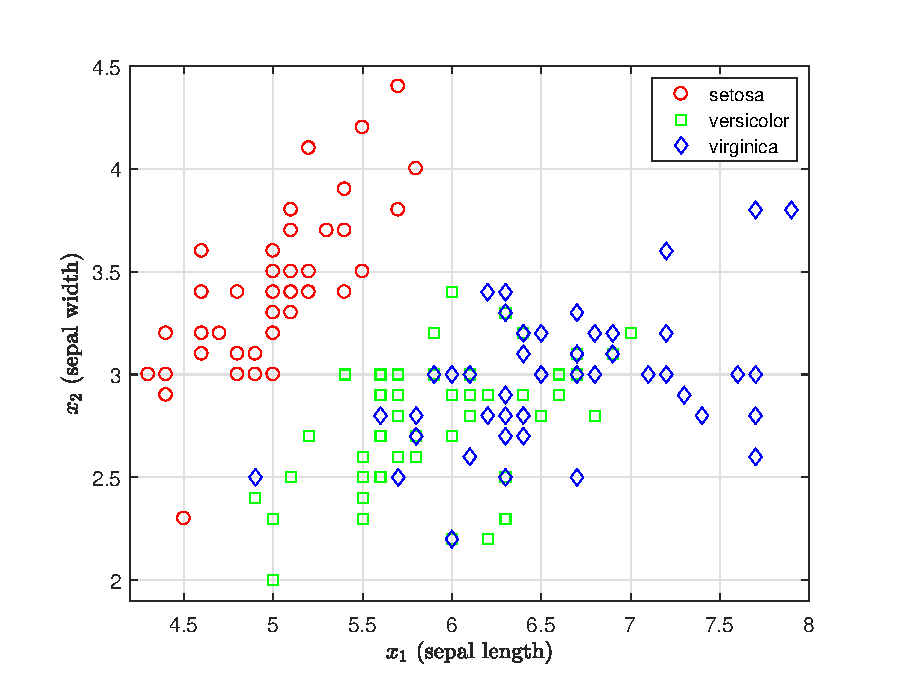
\includegraphics[width=0.7\textwidth]{figures/data.eps}
	\caption{Conjunto de dados \texttt{fcmdata.dat}.}
	\label{fig:fcmdata}
\end{figure}

\begin{figure}[!htbp]
	\centering
	\subfigure[Imagem $01$]{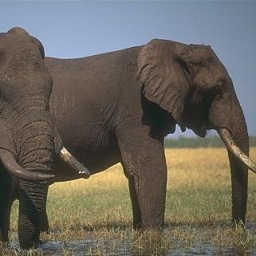
\includegraphics[width = 0.4\textwidth]{figures/img01.jpg}}
	\subfigure[Imagem $02$]{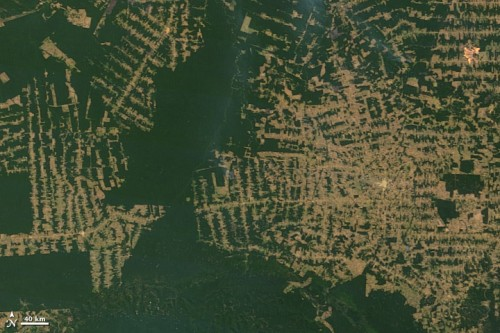
\includegraphics[width = 0.5\textwidth, height = 0.26\textheight]{figures/img02.jpg}}
	\subfigure[Imagem $03$]{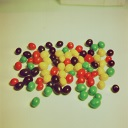
\includegraphics[width = 0.28\textwidth]{figures/img03.jpg}}
	\caption{Imagens usadas na aplicação do algoritmo c-means para segmentação de imagens.}
	\label{fig:images}
\end{figure}

%\subsection{Procedimentos Computacionais}
\section{Resultados}

Nessa seção serão apresentados os resultados dos experimentos descritos anteriormente na Seção \ref{section:descr}.

\subsection{Agrupamento de dados}

O algoritmo \textit{c-means} implementado foi utilizado para agrupamento de dados do conjunto de dados \texttt{fcmdata.dat}, considerando 4 agrupamentos, isto é $c=4$. As Figuras \ref{fig:resul_cluster_cmeans} e \ref{fig:resul_cluster_fcm} ilustram os centros dos agrupamentos obtidos quando utilizado o algoritmo implementado e a função \texttt{fcm} do MATLAB, respectivamente.

\begin{figure}[!htbp]
	\centering
	\subfigure[Algoritmo desenvolvido.]{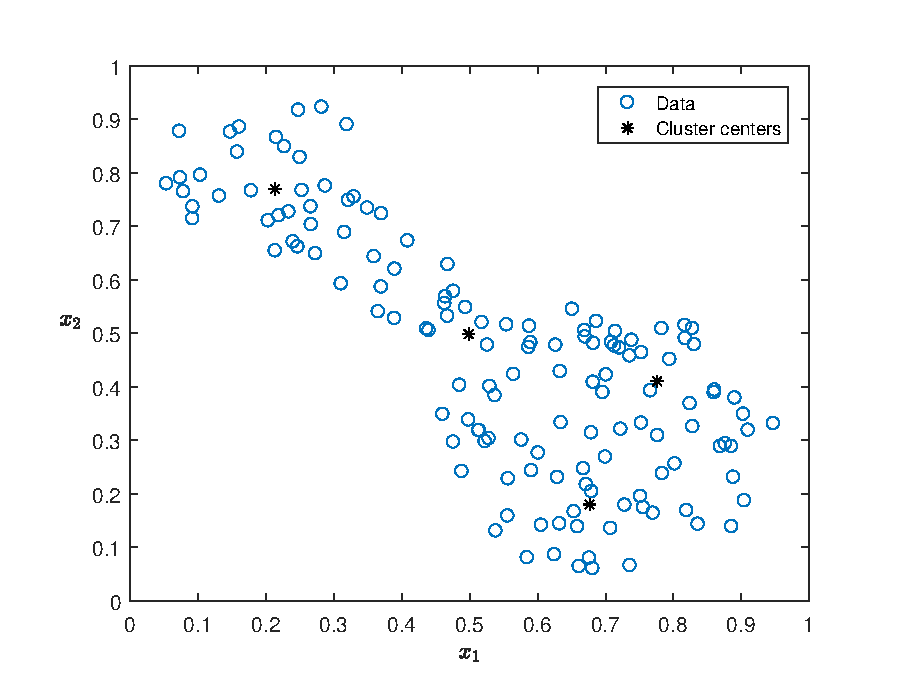
\includegraphics[width = 0.25\textwidth]{figures/data_cmeans.eps}\label{fig:resul_cluster_cmeans}}
	\subfigure[Função \texttt{fcm} do MATLAB.]{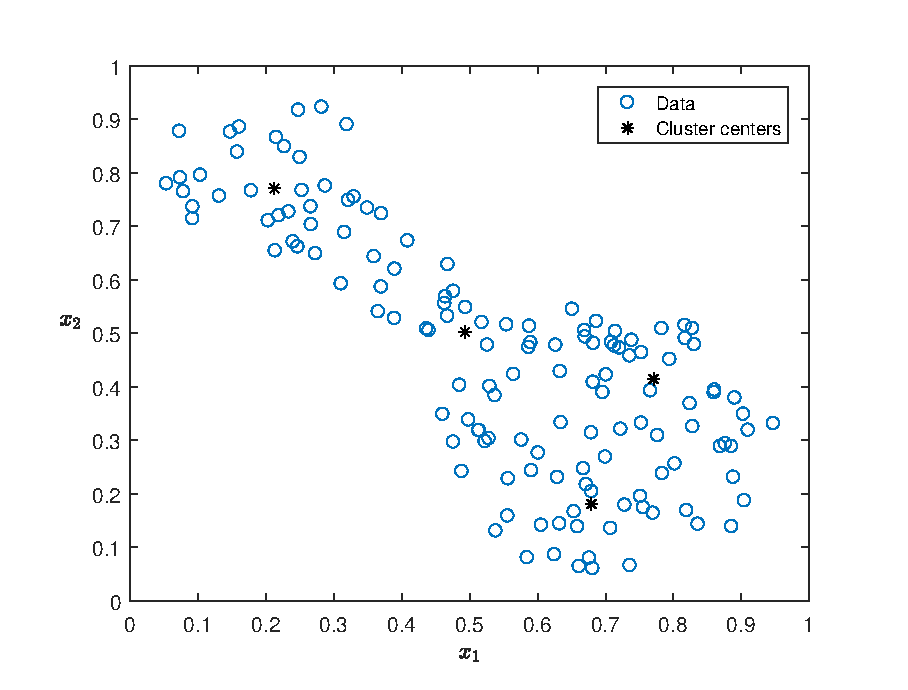
\includegraphics[width = 0.25\textwidth]{figures/data_fcm.eps}\label{fig:resul_cluster_fcm}}
	
	\caption{Comparação dos centros dos agrupamentos, considerando 4 agrupamentos, obtidos por meio do algoritmo c-means implementado e da função \texttt{fcm} do MATLAB.}
\end{figure}

\subsection{Segmentação de imagens}
\label{subsection:seg}

Na abordagem computacional, por meio da técnica de validação cruzada, cada conjunto de espécies foi separado de forma aleatória em subconjuntos de treinamento e validação representados, com dimensão de $70\%$ e $30\%$, respectivamente de cada classe de padrões.

Para todas as classes, no total, quatro dados de entrada aplicados a três espécies, com $50$ amostras. Como ferramenta de aprendizagem, os conjuntos de treinamento e validação, foram determinados observando-se os percentuais em $35$ e $15$ amostras, respectivamente, para cada classe $C_{j}$.

\begin{figure}[!htbp]
	\centering
	\subfigure[$c=2$.]{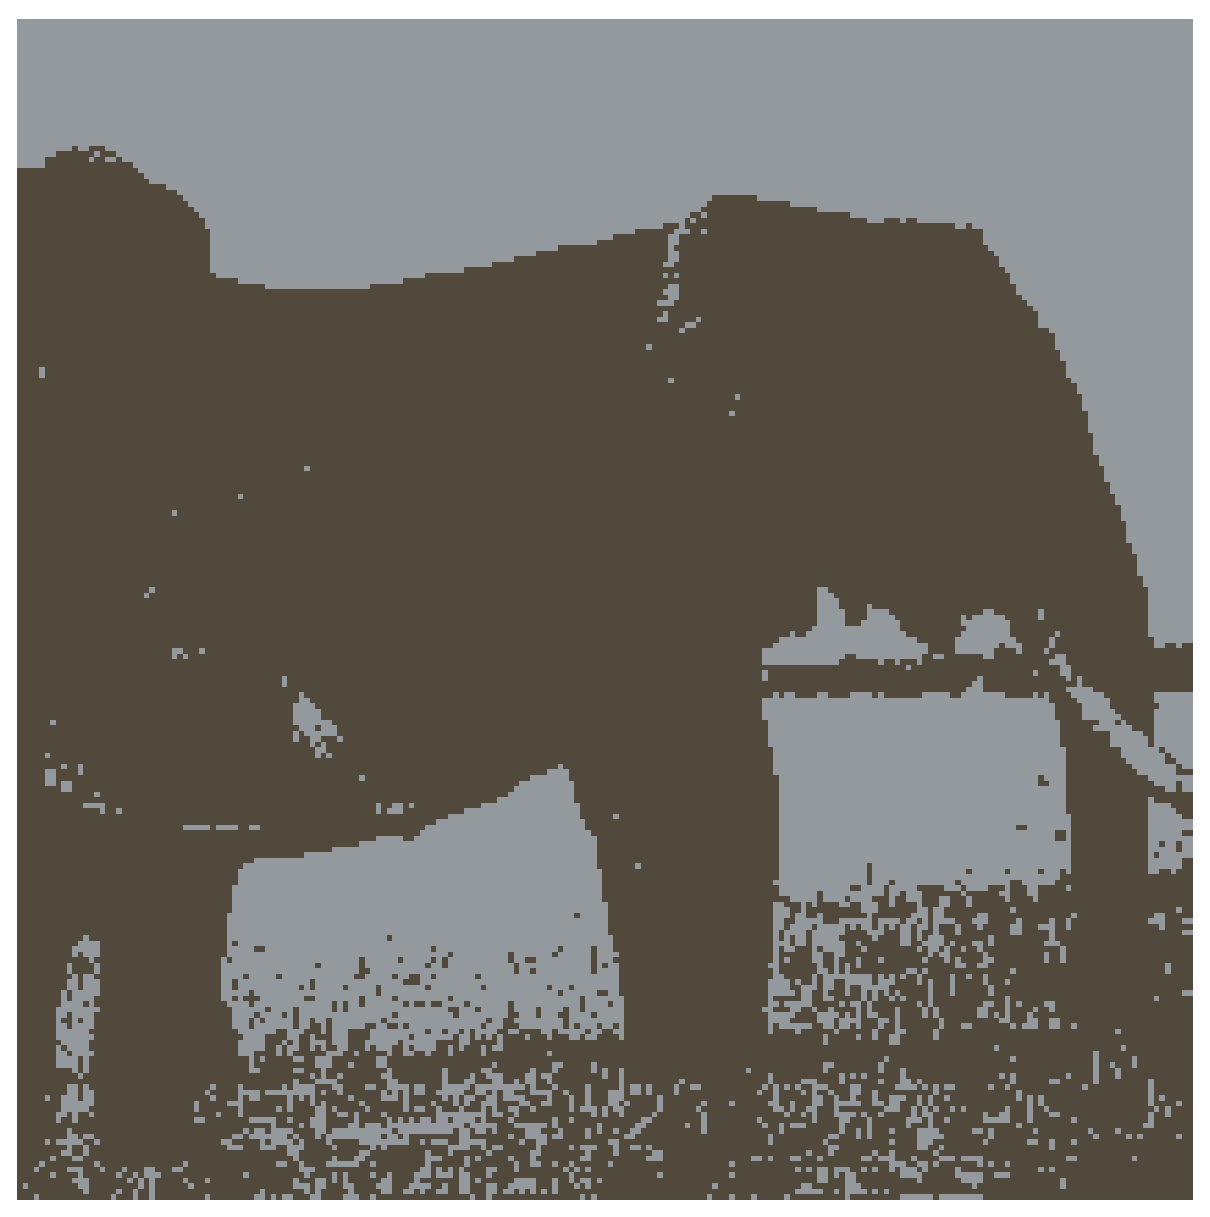
\includegraphics[width = 0.4\textwidth]{figures/img1_2.eps}}
	\subfigure[$c=2$.]{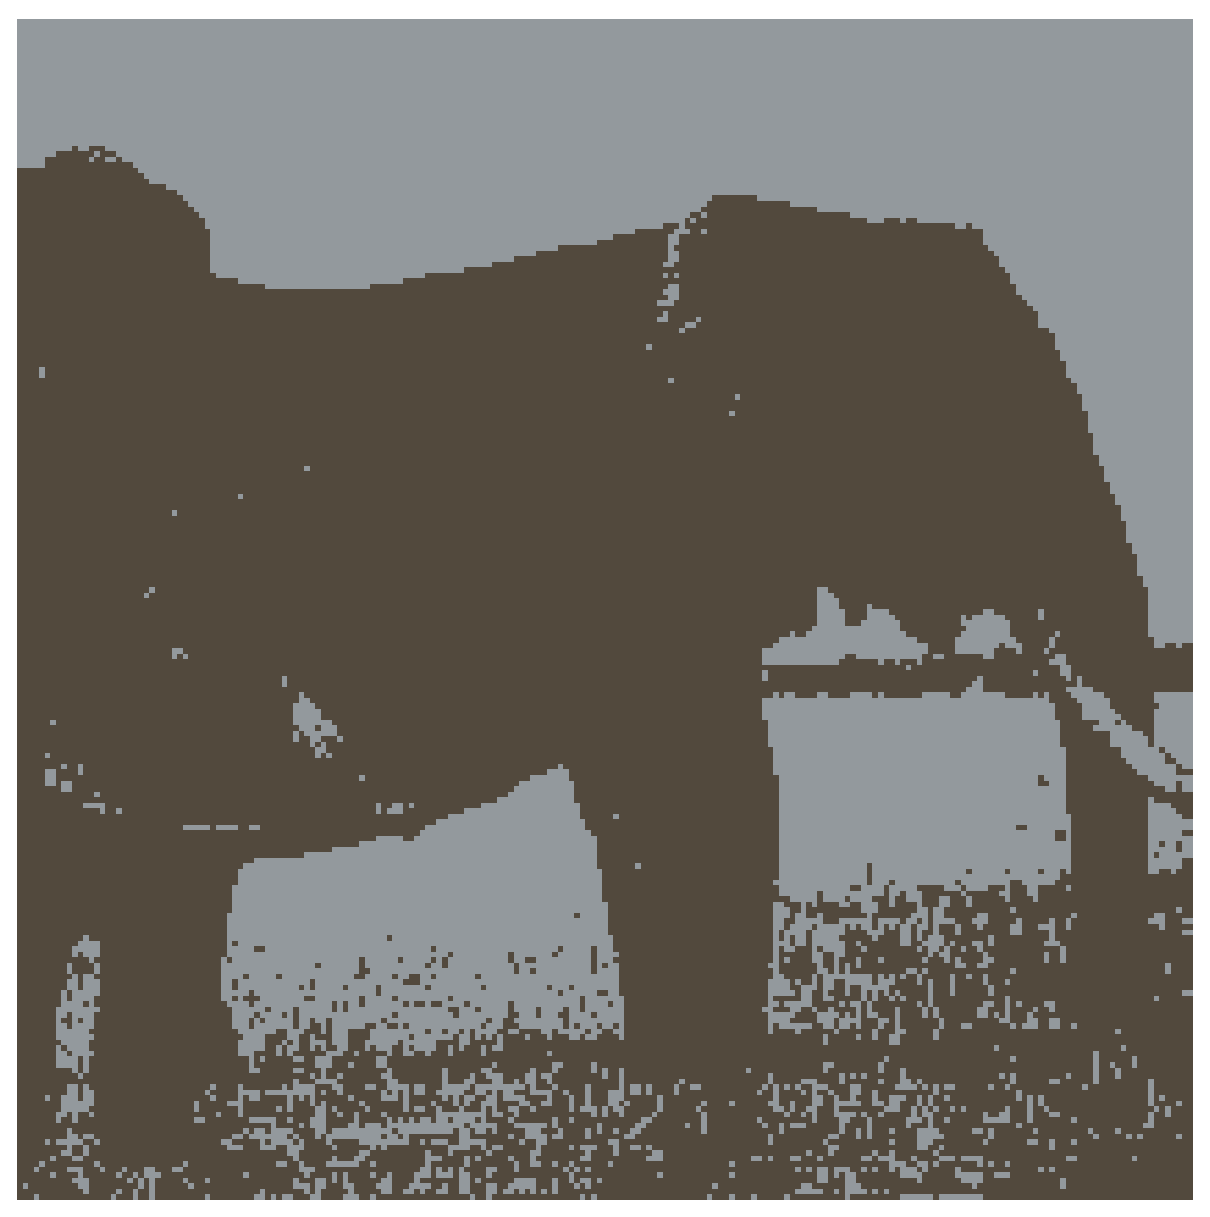
\includegraphics[width = 0.4\textwidth]{figures/matlab_img1_2.eps}}
	
	\caption{Comparação da segmentação da imagem 01 para $2 \leq c \leq 6$, obtidas por meio do algoritmo c-means implementado e da função \texttt{fcm} do MATLAB.}
	\label{fig:resul_img01}
\end{figure}

\newpage
\section{Conclusões}

A utilização de sistemas de classificação baseados em regras ponderadas através de graus de certeza, oferece uma solução baseada em conhecimento dedutivo, o que em termos práticos, implica na sobreposição de uma regra dominante sobre outra no espaço fuzzy, ou seja, na combinação de $n$ regras, pelo menos uma, por inferência composicional, forma a consequência lógica e tendência.

Todos os procedimentos realizados no artigo e replicados nas simulações descritas compõem base de conhecimento por raciocínio aproximado, pelo fato da definição de consequentes a partir de relações de compatibilidade. Neste sentido a conclusão das conjunções lógicas, seja pelo operador mínimo ou produto como \textit{t-norma}, são baseadas no domínio de uma regra sobre a outra no espaço de decisão, sendo este ponderado pelo grau de certeza.

Assim, o procedimento apresentado em [1], o qual consiste na ponderação de regras SE-ENTÃO a partir de graus de certeza substitui a necessidade de otimização das funções de pertinências empregadas para descrição das variáveis linguísticas.
\newpage

\section*{Referências}
\addcontentsline{toc}{section}{\protect\numberline{}Referências}%

[1] ISHIBUCHI, Hisao; NAKASHIMA, Tomoharu. Effect of rule weights in fuzzy rule-based classification systems. IEEE Transactions on Fuzzy Systems, v. 9, n. 4, p. 506-515, 2001.

\end{document}
